\chapter{Introducción}
\label{chapter:introduccion}

\section{Evaluaciones y opiniones}
\label{section:evaluaciones-cruzadas}
\noindent Llamaremos ítem, a un elemento del mundo real que es aprovechado por las personas, dicho ítem puede ser, un objeto, un servicio, una idea, un programa, etc. Además, debería poder ser abstraído a un modelo representado por una computadora, de manera tal, que esa representación describa con precisamente a qué se referie ante la interpretación del lector. 

\noindent Para ello, el modelo del ítem contendrá un conjunto de atributos que lo describen. Algunos más importantes que otros.
\\\\
Por ejemplo, imaginemos que se debe representar una bicicleta mediante un conjunto de pares atributo;valor, tendríamos algo como esto.
\begin{lstlisting}[frame=single] 
Tipo: Bicicleta
Sexo: Unisex
Talle: 51
Cuadro-Material: Aluminio
Cuadro-color: Rojo
Cuadro-Tipo: Ruta
Horquilla-Material: Fibra de carbono
Horquilla-Color: Rojo
Asiento-tipo: Adamo 
Asiento-Color: Blanco
\end{lstlisting}
La cantidad de atributos que pueden utilizarse para describir el ítem puede ampliarse prácticamente hasta el cansancio. 
\\\\
Se pueden optar también por una representación como ésta:
\begin{lstlisting}[frame=single] 
Tipo: Bicicleta
Talle: 51 
Marca: Merida
Modelo: Reacto 500
\end{lstlisting}
Puede aprovecharse el hecho de que es muy probable que ya existan definiciones del ítem que intentamos describir, por lo que si se utilizan sólo los atributos que lo identifican, será suficiente para que el lector tenga la interpretación correcta del mismo. 
\\\\
Cada ítem es de alguna manera utilizado por uno o más usuarios. Y cada usuario puede de la misma manera ser representado en la computadora mediante pares de atributo;valor. Y al igual que los ítems algunos atributos servirán para identificar al usuario. 
\\\\
Definiremos a una reseña (de aquí en adelante review) a la representación mediante la computadora, de la medida de conformidad con respecto a dicha relación entre usuario e ítem. 

Esta relación de uso entre usuario e ítem, contiene un grado de conformidad entre el primero y el segundo, si el ítem cumplió o no con las expectativas del usuario debería poder modelarse también para ser representado computacionalmente.

El objetivo de un review, es que un usuario pueda reflejar el sentimiento que le generó utilizar el ítem e informarlo a otros usuarios. 

También los reviews dispondrán de un conjunto de atributos de los cuales algunos serán indispensables y otros que enriquecerán no sólo su valor intrínseco, sino también su utilidad para el contexto en el que será planteado.
\\\\
Imaginemos un usuario que realiza un review sobre la bicicleta, podría generar el siguiente review:
\begin{lstlisting}[frame=single] 
Puntuacion:4 
Título:``Buena opcion''
Texto:``Liviana y comoda, pero un poco rigida para 
        doblar, y no frena adecuadamente ''
Fecha:15/10/2012
\end{lstlisting}
\begin{figure}
    \centering
    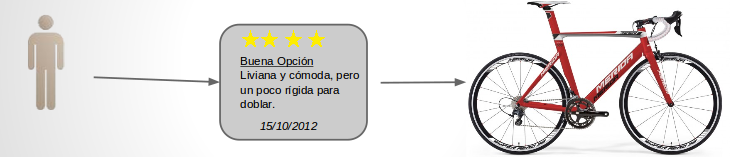
\includegraphics[width=0.8\textwidth,natwidth=610,natheight=642]{biciReview.png}
    \caption{Relación entre usuario, review e ítem}
\end{figure}

La existencia de los reviews en la web es muy importante, ya que dan un panorama socialmente perfeccionado (dado que permiten que no sólo una persona
opine sobre un ítem, lo que da a lugar a muchas evaluaciones y provoca que se acerque al valor real) sobre un ítem, lo que ayuda a 
quienes necesiten una descripción y valoración de los mismos que no provenga de quien los quiere promocionar.

\begin{framed}
\textcolor{red}{Al terminar de leer esta sección, el lector debe entender a que te referís con reviews (en términos generales), que muchas de ellas son publicadas en la web en redes sociales, en sitios de productos etc, y que sirven para ??. Podés agregar algunos ejemplos e incluso imágenes. No queda claro por que en el titulo de la sección dice ``entrecruzadas'', ¿es importante o fue solo una elección al azar?. Para que este se conecte con el que sigue, podés dejar picando algo como ``muchos han intentado procesar automáticamente las opiniones de los usuarios para ... pero eso es muy difícil porque...'' }
\end{framed}


\section{Sistemas de Recomendación}
\label{section:sistemas-de-recomendacion}
\noindent Los sistemas de recomendación son herramientas de software que, en base a un conjunto de ítems (películas, libros, productos, hoteles, etc) e información sobre estos, y un conjunto de usuarios, intentan sugerir ítems apropiados a dichos usuarios. Los sistemas de recomendación se han vuelto una de las herramientas más poderosas para múltiples tipos de aplicaciones web, como comercio electrónico o páginas de noticias. 
\\\\
El desarrollo de estas herramientas, involucra conocimiento en múltiples áreas, como inteligencia artificial, minería de datos, estadística, etc. 
\\\\
Los sistemas de recomendación poseen dos enfoques, el de filtrado colaborativo, y el basado en contenido.
\\\\
Los sistemas de recomendación basados en contenido utilizan un conjunto de informaciones y descripciones de los ítems previamente valorados por un usuario para poder construir un perfil del mismo de manera tal de poder determinar, cuales son sus intereses.

Una vez construido el perfil, pueden procesarse las características de distintos ítems que potencialmente pueden ser recomendados a dicho usuario para determinar si alguno de ellos va acorde al perfil.
\\\\
Los sistemas de recomendación de filtrado colaborativo utilizan la información histórica de cada usuario para intentar encontrar y generar grupos de usuarios con gustos similares. Para lograrlo se compara cada usuario con otro observando qué ítems evaluaron y qué puntajes fueron otorgados. 

De esta forma, si se requiere predecir el interés de un usuario en un ítem, se podrá buscar en dicho grupo de usuarios con gustos similares e inspeccionar aquellos usuarios que hayan realizado un review sobre el ítem.
\\\\
Los sistemas de recomendación de filtrado colaborativo tienen una eficacia superior a los basados en contenido, pero cuentan con una gran desventaja, no permiten predecir intereses para aquellos ítems que aún no poseen evualuaciones, o también para aquellos usuarios que no han evualuado ningún ítem.  A esto se lo llama “arranque en frío”.

\begin{figure}
    \centering
    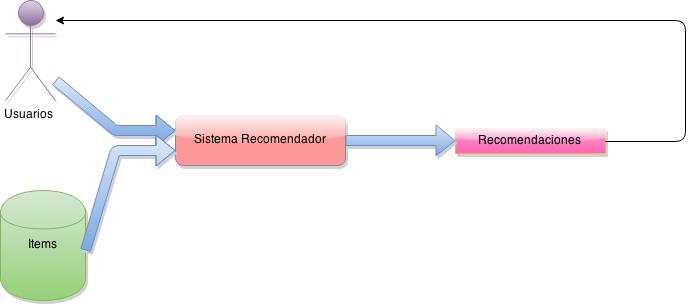
\includegraphics[width=0.8\textwidth,natwidth=610,natheight=642]{recSis}
    \caption{Flujo de un Sistema de Recomendación}
\end{figure}

\section{La web semántica}
\label{section:la-web-semantica}
En sus comienzos en los 90, la web podía verse como un conjunto de sitios web que ofrecían una colección de documentos web interconectados mediante la hipermedia, con el objetivo de comunicar información a los usuarios.
El contenido de esos documentos sólo era generado por el mismo creador y publicador del documento, y los usuarios se limitaban a consumirlo. Por otro lado, era a su vez estático, es decir, se publicaba en la misma forma que se almacenaba y no cambiaba.  
\\\\
Hacia fines de los 90 los sitios web comenzaron a implementar una serie de herramientas (que si bien ya se encontraban disponibles anteriormente no se utilizaban por un problema de performance) que permitieron a los usuarios finalmente participar de la producción del contenido web. Lo que produjo notorios cambios en cuanto a la cantidad de información disponible y proveyó diferentes formas de uso de la web (blogs, redes sociales, canales rss, etc). Más adelante ante la apreciación del pasaje de web estática a una web dinámica, se acuño a esa actual web como web 2.0 y retrónimamente 1.0 a la anterior.
\\\\
Ese cambio provocó un aumento en el tamaño de la web, que se volvió inmenzamente grande, y llevó a la necesidad de implementar tecnologías que ayuden al aprovechamiento de esa cantidad de información. 
Se comenzó entonces a utilizar una serie de frameworks y estándares que permitieron enriquecer (mediante metadatos semánticos y ontológicos dentor de los estándares de la W3C) los datos contenidos en los documentos de manera tal que estos puedan ser consumidos, interpretados y utilizados directamente no sólo por las personas, sino también por las computadoras.
Esto generó que los datos también puedan ser relacionados entre sí, de la misma manera que los documentos son interconectados formando una web de documentos, los datos interconectados forman una web de datos parelela.
Todo este conjunto de actividades frameworks y herramientas forman la ``Web semántica'' que es el puntapié incial para una web mucho más interoperable, lo que permite facilidades para el uso de la web por parte de las aplicaciones y da lugar a otro paso en la evolución de la web, la web 3.0. 
La Web Semántica promete facilitar el desarrollo de la web social y la inteligencia colectiva, a través de mecanismos de clasificación, relación y descripción del contenido de la información publicada mejorando su interoperabilidad. Promete también mejorar la recolección, agregación e integración de datos específicos mediante el uso de agentes de búsqueda automáticos que aprovechan las ventajas.
%Con el correr de los años, múltiples tecnologías se fueron implementando y permitieron el desarrollo de una web mucho más grande y aprovechable...  y esto es unaa referencia a un libro sobre web semantica \cite{Antoniou}

\begin{figure}
    \centering
    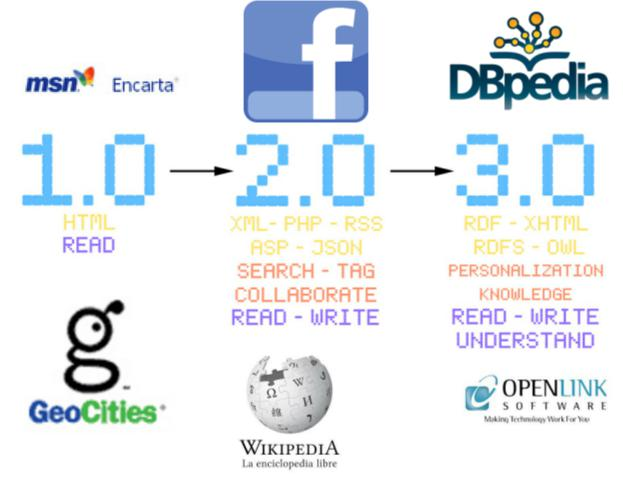
\includegraphics[width=0.8\textwidth,natwidth=610,natheight=642]{webevolve}
    \caption{Evolución de la web}
\end{figure}

\begin{framed}
\textcolor{red}{Al terminar de leer esta sección, el lector debe entender que es la web semántica y a que apunta. Si dejaste picando el tema de automatización en el párrafo anterior, acá se va a imaginar porque hablás de ws. Habla muy bremente de tripletas y meciona RDF. También mencioná linked open data para darle una idea de que la web semantica es una web de datos interconectada. Podés tomar lo que ya escribiste en la propuesta. Ejemplifica con dbpedia o algo asi... En un capitulo mas adelante vas a entrar en detalle en web semantica, rdf, etc. Acá contás solo lo suficiente para que se entienda lo que vas a proponer en la próxima sección}
\end{framed}

\section{Reviews en la web semántica}
\label{section:reviews-en-la-web}

La web 2.0 dio la posibilidad a los usuarios consumidores de la web de generar y publicar contenido en la misma, lo cual cumple con los requerimientos de una plataforma para reviews. Proporciona un entorno para crearlos y publicarlos, lo cual en el caso es una tarea muy sencilla. 
Pero la dificultad de encontrarlos y explotarlos parece ser inversamente proporcional a generarlos. Dado que a mayor facilidad de publicar contenido en la web, mayor se vuelve la inmensidad de la misma y mayor se vuelve la dificultad de encontrar algo dentro de ella.

Veamos dos ejemplos que requieren encontrar reviews en la web:

Imagínense que son ingenieros de Mérida y lanzaron al mercado la bicicleta Reacto 500. Como buenos ingenieros necesitan conocer qué opinan sus clientes, por lo que buscarán reviews en algún motor de búsqueda y luego leerán uno por uno cada review con el objetivo de resumir las opiniones. Humanamente esta tarea demandará mucho tiempo y con un límite corto de cantidad de reviews. 
Ahora peor aún, imagínense que necesitan saber que opina la gente de determinada región (por ejemplo el norte de europa), la tarea de buscar los reviews necesarios se volvería aún más complicada.
Con la posibilidad de contar con una web en la cual los datos son interpretados por las aplicaciones de software y estos a su vez están interconectados, podría crearse una aplicación que pueda automáticamente buscar, clasificar y procesar los reviews para generar automáticamente el resumen.

Ahora bien, si en lugar de requerir reviews de un ítem en particular, se necesitan reviews para una aplicación que recomiende ítems a usuarios, ya no sería una tarea realizable humanamente. Para ello haría falta una aplicación que haga crawling en la web y de alguna manera identifique reviews y a su vez identifique el ítem al cual el review hace referencia. 
Parece algo muy difícil de lograr, salvo que se trabaje sobre sitios conocidos con documentos estructuralmente dominados los cuales se pueda recorrer el DOM automáticamente y acceder a los reviews.
De nuevo, la Web Semántica promete solucionar este problema, con el uso de metadatos que dan información sobre los datos, haciendo que una aplicación pueda fácilmente identificar reviews y navegar por la hipermedia de los datos para conseguir información sobre el ítem y usuario referenciados.

La figura \ref{figure:semanticwebreview} muestra un ejemplo concreto de un review publicado en la web, respetando los lineamientos de la web semántica. 

\begin{figure}
    \centering
    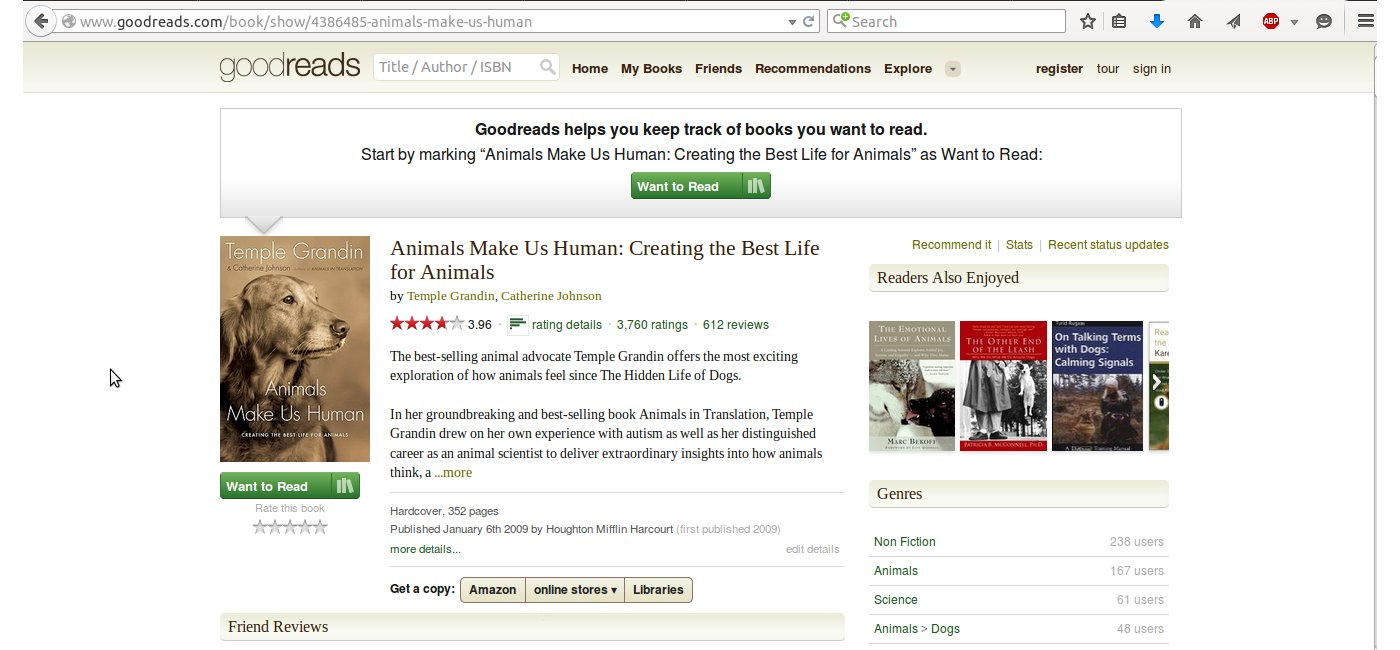
\includegraphics[width=0.8\textwidth,natwidth=610,natheight=642]{semanticwebreview}
    \caption{Ejemplo de review en la web semántica}
    \label{figure:semanticwebreview}
\end{figure}

\begin{framed}
\textcolor{red}{Acá es donde presentas el problema a resolver. Ya contaste que son los reviews y por que alguien querría integrarlos. Ya contaste que es la web semántica y linked open data. Ahora tenés que contar que ha habido iniciativas para darle semántica a los reviews y que existen datos; ahora hay una posibilidad de aprovechar esa información. Y ahí decís algo como lo que dijiste al final de la propuesta: \textit{El objetivo principal de esta tesis es evaluar la viabilidad, y entender los desafíos de la utilización de la información contenida en la web semántica en la construcción de sistemas de recomendación. Para eso, y con foco en el caso particular de opiniones de usuarios sobre distintos tipos de recursos se buscará: capturar, extraer, validar calidad, curar, integrar, publicar y explotar los datos disponibles}.}
\end{framed}

\section{Caso de estudio}
\label{section:caso-de-estudio}
Para mantener en contexto este trabajo, utilizaremos un caso de estudio. Se trata de una aplicación que integra información de reviews disponible en la web semántica para producir recomendaciones simples. En particular, ofrece los siguientes servicios: 

\begin{description}
\item[Rankings de popularidad] Los rankings de popularidad son listas ordenadas... . Para construirlos, se hace necesario obtener y combinar... 
\item[Rankings de popularidad] Los rankings de popularidad son listas ordenadas... . Para construirlos, se hace necesario obtener y combinar... 
 
\end{description}


\section{Organización}
\label{section:organizacion}

\begin{framed}
\textcolor{red}{ya saben lo que vas a contar; acá les das una idea de como te vas a organizar para contarlo - puede ser algo como lo que está a continuación. Para el caso de estudio podés tomar el texto que escribimos en el articulo}
\end{framed}.

 El capítulo \ref{chapter:estrategia} introduce los conceptos de Web Semantica, sus principios y tecnologías y presenta la estrategia de trabajo en términos generales. Los capítulos \ref{chapter:seleccion} a \ref{chapter:explotacion} discuten en detalle cada uno de pasos de la estrategia elegida, aplicándolos al caso de estudio: los reviews en la web semántica. Finalmente, el capítulo \ref{chapter:conclusiones} resumen los resultados observados, saca conclusiones al respecto, y plantea trabajo futuro. El anexo \ref{anexo} presenta una publicación que fue resultado del trabajo efectuado en este trabajo de tesis. 




